\begin{frame}{Motivation}
  Automatische Codegenerierung durch konsistente Modelle

  Allerdings Diskrepanz zwischen Modellierungaspekten:

  \begin{itemize}
    \item \textbf{Strukturmodellierung}
    \begin{itemize}
      \item UML-Klassen- oder Komponentendiagrammen 
    \end{itemize}

    \item \textbf{Verhaltensmodellierung}
    \begin{itemize}
      \item UML-Sequenzdiagrammen oder Petrinetzen
    \end{itemize}
  \end{itemize}
\end{frame}
\begin{frame}{Motivation}
  \begin{figure}
  \centering
  \begin{adjustbox}{width=.7\linewidth,center}
    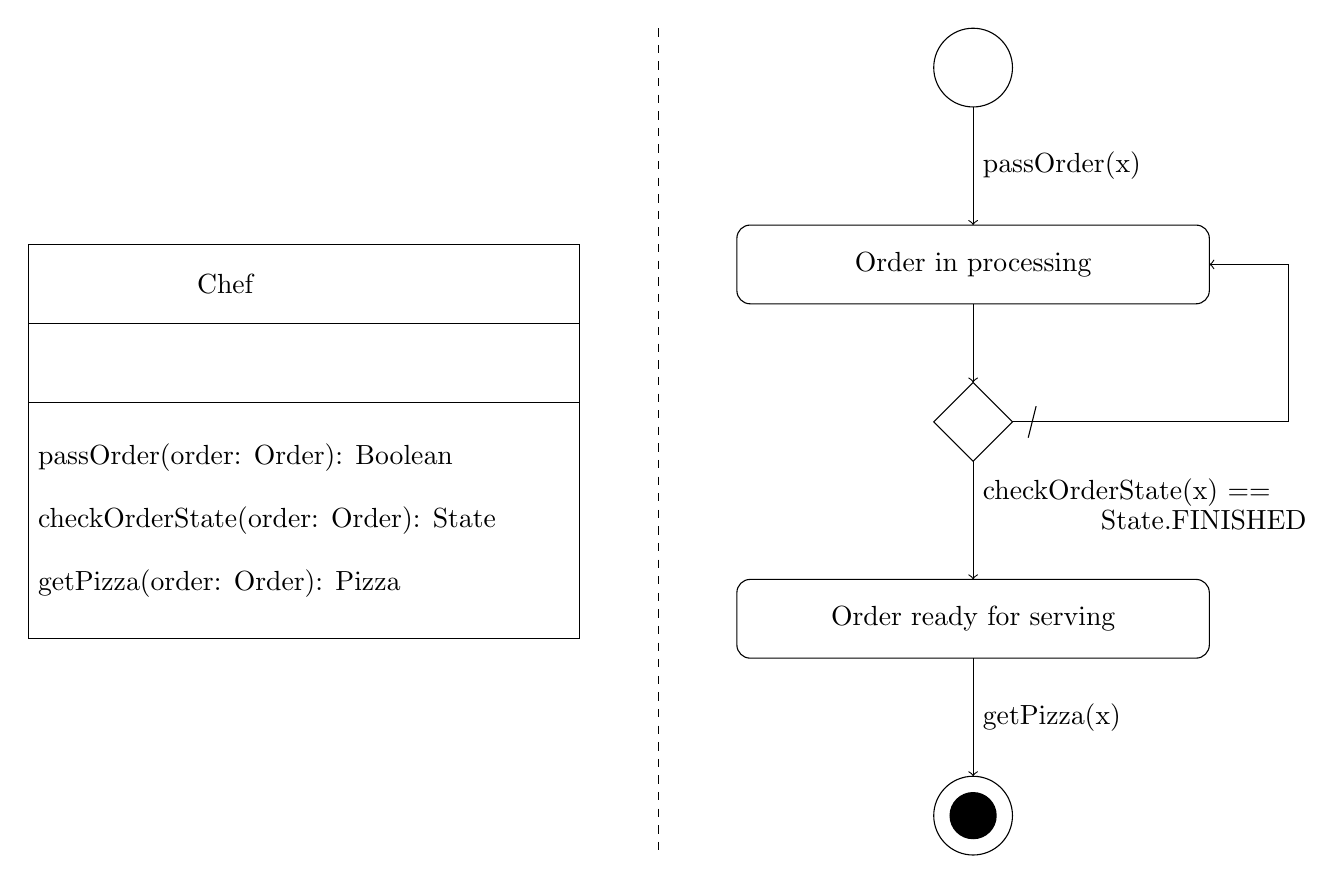
\begin{tikzpicture}
      \draw[dashed] (0,5) -- (0,-5.5);

      \begin{scope}[shift={(0,-0.25)}]
        \draw (-8,2.5) rectangle (-1,-2.5);
        \draw (-8,1.5) -- (-1,1.5);
        \draw (-8,0.5) -- (-1,0.5);
        \draw (-5.5,2) node{Chef};
        \draw (-8,-0.2) node[anchor=west] {passOrder(order: Order): Boolean};
        \draw (-8,-1) node[anchor=west] {checkOrderState(order: Order): State};
        \draw (-8,-1.8) node[anchor=west] {getPizza(order: Order): Pizza};
      \end{scope}

      \draw (4, 4.5) circle[radius=0.5];
      \draw[->] (4,4) -- (4,2.5);
      \draw (4,3.25) node[anchor=west] {passOrder(x)};
      \draw[rounded corners=4.8pt] (1,2.5) rectangle (7,1.5);
      \draw (4,2) node {Order in processing};
      \draw[->] (4,1.5) -- (4,0.5);
      \draw (4,0.5) -- (4.5,0) -- (4,-0.5) -- (3.5,0) -- cycle;
      \draw[->] (4.5,0) -- (8,0)-- (8,2) -- (7,2);
      \draw (4.7,-0.2) -- (4.8,0.2);
      \draw[->] (4,-0.5) -- (4,-2);
      \draw (4,-0.9) node[anchor=west] {checkOrderState(x) ==};
      \draw (5.5,-1) node[anchor=north west] {State.FINISHED};
      \draw[rounded corners=4.8pt] (1,-3) rectangle (7,-2);
      \draw (4,-2.5) node {Order ready for serving};
      \draw[->] (4,-3) -- (4,-4.5);
      \draw (4,-3.75) node[anchor=west] {getPizza(x)};
      \draw (4, -5) circle[radius=0.5];
      \fill (4, -5) circle[radius=0.3];
    \end{tikzpicture}
  \end{adjustbox}
\end{figure}

\end{frame}
\begin{frame}{Motivation}
  \begin{figure}
  \centering
  \begin{adjustbox}{width=.75\linewidth,center}
    \begin{tikzpicture}
      \draw[dashed] (0,4.7) -- (0,-5.2);

      \begin{scope}[shift={(0,-0.25)}]
        \draw (-8,2.5) rectangle (-1,-2.5);
        \draw (-8,1.5) -- (-1,1.5);
        \draw (-8,0.5) -- (-1,0.5);
        \draw (-4.5,2) node{Chef};
        \draw (-8,-0.2) node[anchor=west] {passOrder(order: Order): Bool};
        \filldraw[fill=error!10,draw=error] (-7.95, -0.6) rectangle (-1.05,-1.4);
        \draw (-8,-1) node[anchor=west,color=error] {\underline{isOrderFinished}(order: Order): \underline{Bool}};
        \draw (-8,-1.8) node[anchor=west] {getPizza(order: Order): Pizza};
      \end{scope}

      \draw (4, 4.2) circle[radius=0.5];
      \draw[->] (4,3.7) -- (4,2.5);
      \draw (4,3.1) node[anchor=west] {passOrder(x)};
      \draw[rounded corners=4.8pt] (1,2.5) rectangle (7,1.5);
      \draw (4,2) node {Order in processing};
      \draw[->] (4,1.5) -- (4,0.5);
      \draw (4,0.5) -- (4.5,0) -- (4,-0.5) -- (3.5,0) -- cycle;
      \draw[->] (4.5,0) -- (8,0)-- (8,2) -- (7,2);
      \draw (4.7,-0.2) -- (4.8,0.2);
      \draw[->] (4,-0.5) -- (4,-2);
      \filldraw[fill=error!10,draw=error] (4.05, -0.5) rectangle (8.45,-1.65);
      \draw (4,-0.9) node[anchor=west,color=error] {checkOrderState(x) ==};
      \draw (5.5,-1) node[anchor=north west,color=error] {State.FINISHED};
      \draw[rounded corners=4.8pt] (1,-3) rectangle (7,-2);
      \draw (4,-2.5) node {Order ready for serving};
      \draw[->] (4,-3) -- (4,-4.2);
      \draw (4,-3.6) node[anchor=west] {getPizza(x)};
      \draw (4, -4.7) circle[radius=0.5];
      \fill (4, -4.7) circle[radius=0.3];

      \draw[dashed,color=layer3,line width=0.025cm] (-1,-0.45) -- (0.5,-0.45) -- (0.5,3.1) -- (4,3.1);
      \draw[dashed,color=error,line width=0.03cm] (-1,-1.25) -- (1,-1.25) -- (1,-1.1) -- (4,-1.1);
      \draw[dashed,color=layer3,line width=0.025cm] (-1,-2.05) -- (0.5,-2.05) -- (0.5,-3.6) -- (4,-3.6);

      \begin{scope}[shift={(2,-1.05)}, scale=0.5]
        \draw[color=error,line width=0.05cm, -{Triangle[width=0.13cm]}] (0.2,0.5) -- (-0.2,-0.1) -- (0.2,0.1) -- (-0.27,-0.7);
      \end{scope}
    \end{tikzpicture}
  \end{adjustbox}
\end{figure}

\end{frame}

\begin{frame}{Problemdefinition}
  Bestehende Verfahren zur Konsistenzprüfung:
  \begin{itemize}
    \item UML-Klassendiagramm und UML-Zustandsdiagramm
    
    \item \dots
  \end{itemize}

  Gilt nicht für die Konsistenz zwischen \textbf{BPMN} und \textbf{BROS}:

  \begin{itemize}
    \item Es existieren noch keine Konsistenzbeziehungen

    \item Damit auch kein automatisierbares Verfahren zur Konsistenzprüfung
  \end{itemize}
\end{frame}

\begin{frame}{Forschungsfragen}
  \begin{description}[4cm]
    \item[F1] Welche Konsistenzbeziehungen bestehen zwischen BPMN- und BROS-Modellen?

    \item[F2] Wie lassen sich die Konsistenzbedingungen automatisiert überprüfen?

    \item[F3] Mit welchem Aufwand ist dieses Verfahren erweiterbar?
  \end{description}
\end{frame}
